\chapter{Espaços Vetoriais}
Começaremos pela definição de um espaço vetorial utilizando aquelas apresentadas por \cite{boldrini1980} e \cite{ulhoa2018}, onde, podemos tratar como um vetor ao designar um elemento do espaço vetorial de um número $\mathbb{R}$ definido tal que:

\noindent\textbf{Definição 01:} Seja um conjunto V, não vazio, com duas operações: soma, $(v_1, v_2) \rightarrow v_1 + v_2$, e multiplicação por escalar, $(k, v) \rightarrow kv$, tais que, para quaisquer $u, v, w \in \mathbf{V}$ e $a, b \in \mathbb{R}$, satisfaçam as propriedades: \nocite{boldrini1980}

\begin{enumerate}
	\item $1u = u$.
	\item $\exists$ $0$ $\in V$ tal que $u + 0 = u$.
	\item $\exists$ $-u \in V$ tal que $u + (-u) = 0$.
	\item $a(u + v) = au + av$.
	\item $(a + b)v = av + bv$.
	\item $(ab)v = a(bv)$.
\end{enumerate}

\noindent\textbf{Observação:} $\textbf{0}$ é o vetor nulo. \nocite{ulhoa2018}

\noindent\textbf{Observação:} Limitaremos nossa discussão, demonstrações e aplicações dentro do conjunto dos números reais apenas.

\noindent\textbf{Exemplo 01:} Suponhamos dois pontos no plano, o ponto $\mathbf{O}_{(0, 0)}$ sendo a origem e $\mathbf{M}_{(2, 2)}$, onde, se $\vb{V}$, é um conjunto não vazio e possui a soma desses dois pontos ($\mathbf{O}_{(0, 0)}$ e $\mathbf{M}_{(2, 2)}$). Além disso, seu escalar pertencente ao conjunto dos $\mathbb{R}$, que satisfazem todas as propriedades de um espaço vetorial. Logo $\vb{V}$ é um espaço vetorial.

\begin{figure}[H]
	\centering
	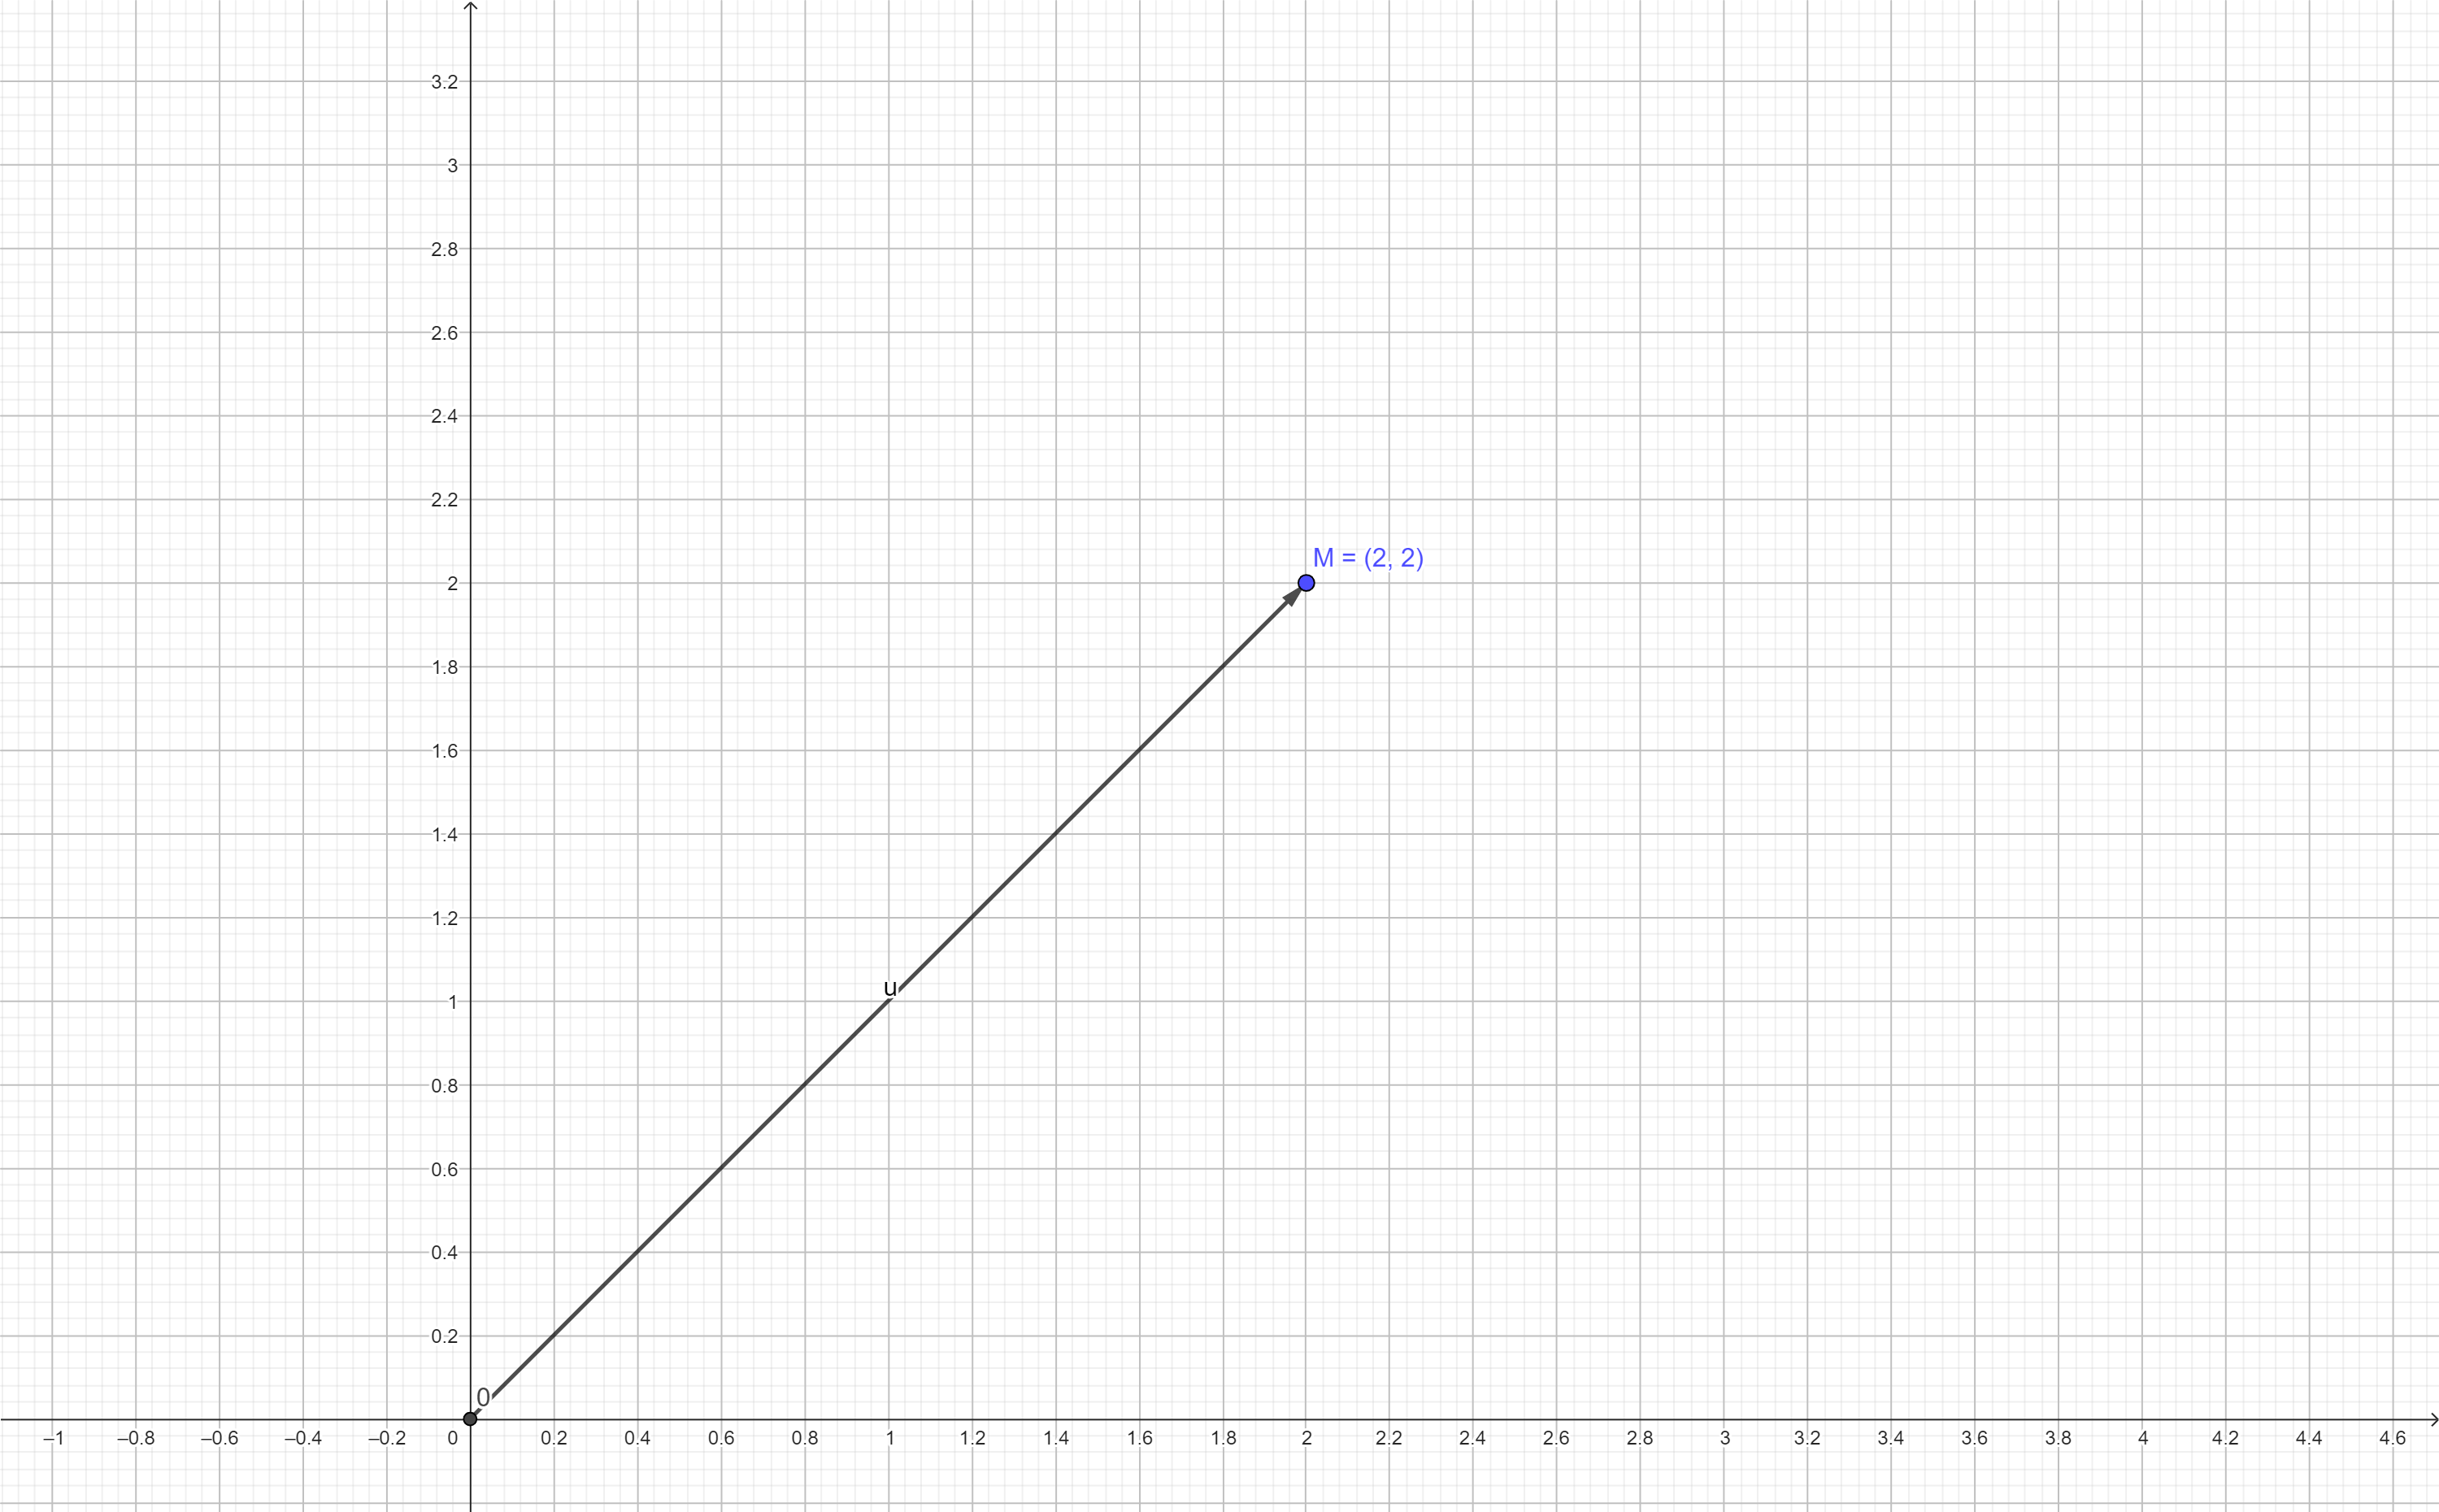
\includegraphics[scale=2.00]{exemplo01.png}
	\caption{Um vetor no plano.}
\end{figure}

A partir disto, podemos perceber o uso analítico dos espaços vetoriais para resolução de problemas em geral. Vejamos mais alguns exemplos.

\noindent\textbf{Exemplo 02:} O exemplo anterior, trata-se de uma matriz de $\mathbb{R}^2$ pode ser dito como, no plano, agora iremos expandir para $\mathbb{R}^3$, seja um vetor $A = (x, y, z)$ ou representado pela forma matricial:

\[
A = \begin{bmatrix}
	a \\ b \\ c
\end{bmatrix}
\]
\noindent Assim, por quaisquer números reais, podemos fazer uma projeção ortogonal no espaço, segue um exemplo traçado:

\begin{figure}[H]
	\centering
	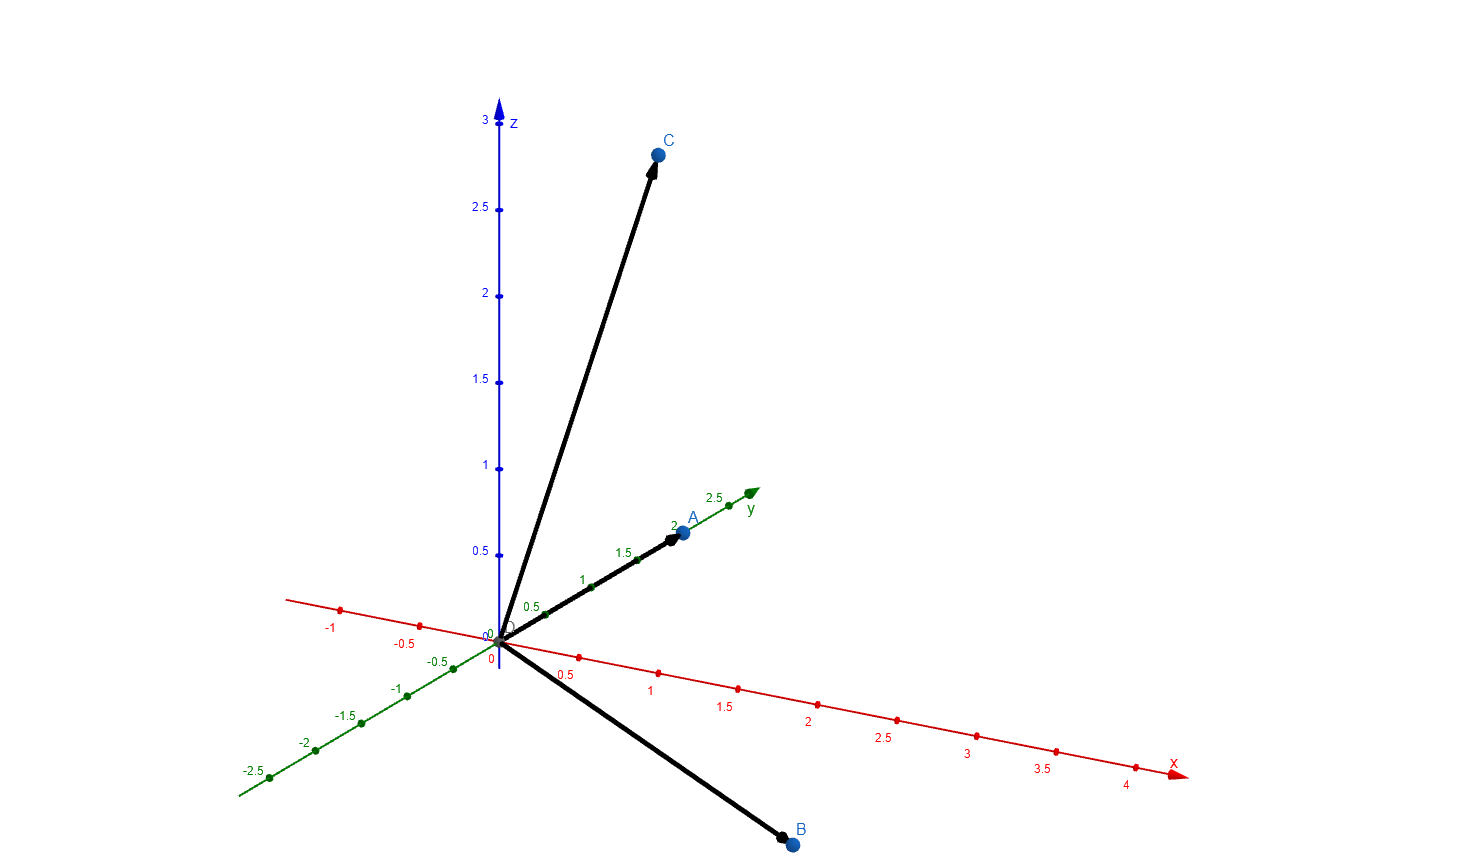
\includegraphics[scale=0.30]{exemplo02.png}
	\caption{Exemplo de vetor no espaço.}
\end{figure}

\noindent\textbf{Exemplo 03:} Consideremos $n-uplas$ de números reais.

\begin{equation}
	V = \mathbb{R}^n = \{(x_1, x_2, \ldots, x_n); x_i \in \mathbb{R}\}
\end{equation}

\noindent e se \( u = (x_1, x_2, \ldots, x_n) \), \( v = (y_1, y_2, \ldots, y_n) \) e \( a \in \mathbb{R} \),

\[
u + v = (x_1 + y_1, x_2 + y_2, \ldots, x_n + y_n) \quad \text{e} \quad a u = (ax_1, ax_2, \ldots, ax_n)
\]


Por tratarmos de uma quantidade $n$ de números, o campo tridimensional deixa de ser visto, e passamos a ter $\mathbb{R}^n$ dimensões, as propriedades não deixam de valer independente a quantidade de dimensões.

\section{Subespaços Vetoriais}
Nesta seção iremos introduzir conceitos no estudo de espaço vetorial para subespaço vetorial.

\noindent\textbf{Definição 02:} Dado um espaço vetorial $\vb{V}$, um subconjunto $\vb{W}$, não vazio, será um subespaço vetorial de $\vb{V}$ se:
\begin{enumerate}
	\item Para quaisquer $u, v \in \vb{W}$ tivermos $u + v \in \vb{W}$.
	\item Para quaisquer $a \in \mathbb{R}, u \in \vb{W}$ tivermos $au \in \vb{W}$.
	\end{enumerate}

\noindent\textbf{Teorema 01:} Um subconjunto não vazio $\vb{W}$ de $\vb{V}$ é um subespaço de $\vb{V}$ se, e somente se, para cada par de vetores $\vec{u}, \vec{v}$ em $\vb{W}$ e cada escalar $\alpha$ em $\mathbb{R}$, o vetor $\alpha\vec{u} + \vec{v}$ está em $\vb{W}$.

\noindent\textbf{Demonstração:} Suponhamos que $\vb{W}$ seja um subconjunto não vazio de $\vb{V}$, tal que, $\alpha\vec{u} + \vec{v}$ pertença a $\vb{W}$ para todos os vetores $\vec{u}, \vec{v}$ em $\vb{W}$ e todos escalares $\alpha$ em $\mathbb{R}$. Como $\vb{W}$ é não vazio, existe um vetor $\vec{w}$ em $\vb{W}$, logo $(-1) \vec{w} + \vec{w} = 0$ está em $\vb{W}$. Então se $\vec{u}$ é um vetor arbitrário em $\vb{W}$ e $\alpha$ é um escalar arbitrário, o vetor $\alpha\vec{u} = \alpha\vec{u} + 0$ está em $\vb{W}$. Em particular $(-1)\vec{u} = -\vec{u}$ está em $\vb{W}$. Finalmente se $\vec{u}$ e $\vec{v}$ estão em $\vb{W}$, então $\vec{u} + \vec{v} = 1\vec{u} + \vec{v}$ está em $\vb{W}$.
Assim, $\vb{W}$ é um subespaço de $\vb{V}$. \nocite{hoffman1979}

\noindent\textbf{Exemplo 04:} Considere o espaço vetorial $\mathbb{R}^3$. O conjunto de todos os vetores que residem no plano $xy$, ou seja, $\{(x, y, 0) \mid x, y \in \mathbb{R}\}$, forma um subespaço vetorial de $\mathbb{R}^3$.

Se o conjunto dado forma um subespaço vetorial de $\mathbb{R}^3$, precisamos verificar as três propriedades fundamentais:

\begin{enumerate}
    \item Contém o vetor nulo: O vetor nulo em $\mathbb{R}^3$ é $(0,0,0)$. Este vetor também está contido no plano $xy$, pois $z = 0$.
    
    \item É fechado sob adição: Se tomarmos dois vetores $(x_1, y_1, 0)$ e $(x_2, y_2, 0)$ no plano $xy$, a sua soma será $(x_1 + x_2, y_1 + y_2, 0)$, que também reside no plano $xy$.
    
    \item É fechado sob multiplicação por escalar: Para qualquer escalar $c$ e vetor $(x, y, 0)$ no plano $xy$, $c \cdot (x, y, 0) = (cx, cy, 0)$, que também está no plano $xy$.
\end{enumerate}

Então, o conjunto de todos os vetores $(x, y, 0)$ com $x, y \in \mathbb{R}$ forma um subespaço vetorial de $\mathbb{R}^3$.

\noindent\textbf{Exemplo 05:} No espaço vetorial das funções reais de uma variável real, $V = \{f(x) \mid f: \mathbb{R} \rightarrow \mathbb{R}\}$, considere o conjunto de todas as funções lineares, ou seja, $\{f(x) = mx + b \mid m, b \in \mathbb{R}\}$. Esse conjunto forma um subespaço vetorial de $V$. Novamente, você pode verificar as propriedades para confirmar.

Se o conjunto dado forma um subespaço vetorial de $V$, novamente precisamos verificar as três propriedades fundamentais:

\begin{enumerate}
    \item Contém a função nula: A função nula em $V$ é $f(x) = 0$. Esta função é uma função linear, pois pode ser escrita como $f(x) = 0 \cdot x + 0$. Portanto, a função nula está contida no conjunto.
    
    \item É fechado sob adição: Se tomarmos duas funções lineares $f_1(x) = m_1x + b_1$ e $f_2(x) = m_2x + b_2$, a sua soma será $f_1(x) + f_2(x) = (m_1 + m_2)x + (b_1 + b_2)$, que também é uma função linear. Portanto, o conjunto é fechado sob adição.
    
    \item É fechado sob multiplicação por escalar: Para qualquer escalar $c$ e função linear $f(x) = mx + b$, a multiplicação por escalar $cf(x) = c(mx + b) = (cm)x + (cb)$ também é uma função linear. Assim, o conjunto é fechado sob multiplicação por escalar.
\end{enumerate}

Portanto, o conjunto de todas as funções lineares $f(x) = mx + b$ com $m, b \in \mathbb{R}$ forma um subespaço vetorial de $V$.

\noindent\textbf{Exemplo 06:} No espaço das matrizes reais $2 \times 2$, $M_{(2,2)}$, considere o conjunto de todas as matrizes simétricas, ou seja, aquelas em que $A = A^T$. Esse conjunto forma um subespaço vetorial de $M_{(2,2)}$. Você pode demonstrar isso verificando as propriedades de um subespaço vetorial

Para tal, é imperativo investigar as três propriedades basilares:

\begin{enumerate}
    \item \textbf{Presença da Matriz Nula:} A matriz nula em $M_{(2,2)}$ é a matriz $\begin{pmatrix} 0 & 0 \\ 0 & 0 \end{pmatrix}$. Nota-se que esta matriz é simétrica, posto que $A = A^T$. Portanto, a matriz nula está asseguradamente contida no conjunto em questão.
    
    \item \textbf{Fechamento sob Adição:} Considerando duas matrizes simétricas $A$ e $B$, a sua soma $A + B$ é também simétrica, visto que $(A + B)^T = A^T + B^T = A + B$. Logo, o conjunto demonstra ser fechado sob adição.
    
    \item \textbf{Fechamento sob Multiplicação por Escalar:} Para qualquer escalar $c$ e matriz simétrica $A$, a multiplicação por escalar $cA$ é igualmente simétrica, haja vista que $(cA)^T = cA^T = cA$. Deste modo, o conjunto revela-se fechado sob multiplicação por escalar.
\end{enumerate}

Assim sendo, constata-se que o conjunto de todas as matrizes simétricas configura-se como um subespaço vetorial de $M_{(2,2)}$.

\section{Combinação Linear}
Dentro de um espaço vetorial, conforme demonstrado que podemos ter subconjuntos de espaços vetoriais, é possível a obtenção de novos vetores a partir de vetores dados \cite{boldrini1980}.

\noindent\textbf{Definição 03:} Sejam $V$ um espaço vetorial, $v_1, v_2, \ldots, v_n \in V$ e $a_1, \ldots, a_n \in \mathbb{R}$. Então, o vetor $v = a_1v_1 + a_2v_2 + \ldots + a_nv_n$ é um elemento de $V$ podendo ser chamado combinação linear de $v_1, \ldots, v_n$.


Seja \( V \) um subespaço de \( W \) (\( V \subset W \)). Se \( W \) é gerado pelos vetores \( v_1, \ldots, v_n \), podemos adotar a notação \( W = [v_1, \ldots, v_n] \). Isso significa que \( W \) é o conjunto de todas as combinações lineares dos vetores \( v_1, \ldots, v_n \). A notação expandida é:

\begin{equation}
	W = [v_1, \ldots, v_n] = \left\{ v \in W \;\middle|\; v = a_1v_1 + \ldots + a_nv_n, \; a_i \in \mathbb{R}, \; 1 \leq i \leq n \right\}
\end{equation}


\noindent\textbf{Exemplo 07:} Presuma um vetor $V = \mathbb{R}^3, v \in V, v \neq 0$. Se imaginarmos sua reta que contém o vetor $v$, onde, $[v] = {av: a \in \mathbb{R}}$

\begin{figure}[H]
	\centering
	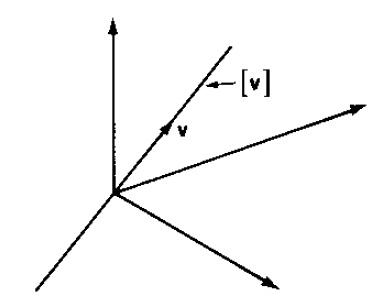
\includegraphics[scale=0.90]{cb_exemplo7.png}
	\caption{Combinação linear de Vetores \cite{boldrini1980}, pg. 113.}
\end{figure}

\noindent\textbf{Exemplo 08:} Se obtemos $v_1, v_2 \in \mathbb{R}^3$ e $v_3 \in [v_1, v_2]$, então $[v_1, v_2, v_3] = [v_1, v_2]$, então $v_3$ é um combinação linear de  $v_1$ e $v_2$.

\begin{figure}[H]
	\centering
	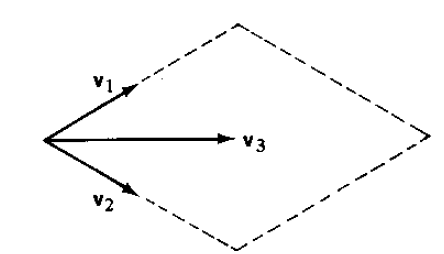
\includegraphics[scale=0.90]{cb_exemplo8.png}
	\caption{Combinação de três vetores lineares \cite{boldrini1980}, pg. 113.}
\end{figure}

\noindent\textbf{Exemplo 09:} Consideremos o espaço vetorial $\mathbb{R}^3$ e os vetores $\mathbf{v} = \begin{pmatrix} 2 \\ 3 \\ 1 \end{pmatrix}$ e $\mathbf{w} = \begin{pmatrix} 1 \\ -1 \\ 2 \end{pmatrix}$. Sejam também os escalares $a = 3$ e $b = -1$. Então temos, os seguintes elementos.

\begin{table}[h]
	\centering
	\begin{tabular}{@{}ccc@{}}
		\toprule
		\textbf{Vetor} & \textbf{Componentes} & \textbf{Escalar} \\ \midrule
		$\mathbf{v}$   & $ 2, 3, 1$   & $3$              \\
		$\mathbf{w}$   & $ 1, -1, 2$  & $-1$             \\ \bottomrule
	\end{tabular}
	\caption{Vetores e escalares utilizados na combinação linear}
\end{table}

Definimos a combinação linear dos vetores $\mathbf{v}$ e $\mathbf{w}$ como:

\begin{equation}
	a\mathbf{v} + b\mathbf{w} = 3 \begin{pmatrix} 2 \\ 3 \\ 1 \end{pmatrix} + (-1) \begin{pmatrix} 1 \\ -1 \\ 2 \end{pmatrix}.
\end{equation}

Aplicando as operações, obtemos:

\begin{equation}
	a\mathbf{v} + b\mathbf{w} = \begin{pmatrix} 6 \\ 9 \\ 3 \end{pmatrix} + \begin{pmatrix} -1 \\ 1 \\ -2 \end{pmatrix} = \begin{pmatrix} 6 - 1 \\ 9 + 1 \\ 3 - 2 \end{pmatrix} = \begin{pmatrix} 5 \\ 10 \\ 1 \end{pmatrix}.
\end{equation}

Portanto, a combinação linear dos vetores $\mathbf{v}$ e $\mathbf{w}$ com os coeficientes $a = 3$ e $b = -1$ é o vetor 

\[
\begin{pmatrix} 5 \\ 10 \\ 1 \end{pmatrix}
\]


\section{Dependência e Independência Linear}
Dado a combinação linear, devemos saber, a priori, se algum desses vetores não é combinação linear dos outros e assim por diante. Para isto precisamos saber sua dependência e independência linear.\nocite{camargo2005}

\noindent\textbf{Definição 03:} Sejam $\mathbf{V}$ um espaço vetorial e $\mathbf{v}_1, \ldots, \mathbf{v}_n \in \mathbf{V}$. Dizemos que o conjunto ${\mathbf{v}_1, \ldots, \mathbf{v}_n}$ é linearmente independente (\textbf{LI}), ou que os vetores $\mathbf{v}_1, \ldots, \mathbf{v}_n$ são \textbf{LI}, se a equação

\begin{equation}
	a_1\mathbf{v}_1 + \ldots + a_n\mathbf{v}_n = 0
\end{equation}

\noindent implica que $a_1 = a_2 = \ldots = a_n = 0$. No caso em que exista algum $a_i \neq 0$ dizemos que ${v_1, \ldots, v_n}$ é linearmente dependente (\textbf{LD}), ou que os vetores $\mathbf{v}_1, \ldots, \mathbf{v}_n$ são \textbf{LD}.

\noindent\textbf{Teorema 02:} Um conjunto de vetores é linearmente dependente (\textbf{LD}) se, e somente se, pelo menos um dos vetores pode ser escrito como uma combinação linear dos outros. Logo,

\begin{equation}
\{\mathbf{v}_1, \ldots, \mathbf{v}_n \} \text{ é \textbf{LD}} \iff \exists i \in \{1, \ldots, n\} \text{ tal que } \mathbf{v}_i = \sum_{j \neq i} c_j \mathbf{v}_j \text{ para alguns } c_j \in \mathbb{R}
\end{equation}

\noindent\textbf{Demonstração:} Sejam $\mathbf{v}_1, \ldots, \mathbf{v}_n$ \textbf{LD} e $a_1\mathbf{v}_1 + \ldots + a_j\mathbf{v}_j + \ldots + a_n\mathbf{v}_n = 0$

\noindent Um dos coeficientes deve ser diferente de zero. Suponhamos que seja $a_j \neq 0$. Então 

\begin{equation}
	\mathbf{v}_j = -\frac{1}{a_j}(a_1\mathbf{v}_1 + \ldots + a_{j - 1}\mathbf{v}_{j - 1} + a_{j + 1}\mathbf{v}_{j + 1} + \ldots + a_n\mathbf{v}_n)
\end{equation}

\noindent e portanto $\mathbf{v}_j = -\frac{a_1}{a_j}\mathbf{v}_1 + \ldots -\frac{a_n}{a_j}\mathbf{v}_n$

\noindent Logo, $\mathbf{v}_j$ é uma combinação linear dos outros vetores.

\noindent\textbf{Exemplo 10:} Sejam $\mathbf{V} = \mathbb{R}^3$ e $v_1, v_2 \in \mathbf{V}$, $\{\mathbf{v}_1, \mathbf{v}_2\}$ é \textbf{LD} $\iff \mathbf{v}_1$ e $\mathbf{v}_2$ estiverem na mesma reta, que passa pela origem. $(\mathbf{v}_1 = \lambda\mathbf{v}_2)$.

\begin{figure}[H]
	\centering
	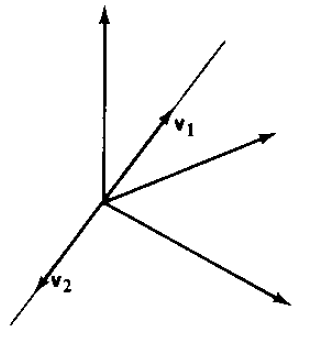
\includegraphics[scale=0.90]{cb_exemplo10.png}
	\caption{Vetores linearmente dependentes \cite{boldrini1980}, pg. 115.}
\end{figure}

\section{Base}
Seja $\mathbf{V}$ um espaço vetorial. Uma base para $\mathbf{V}$ é um conjunto finito $B = \{\mathbf{u}_1, \ldots, \mathbf{u}_n\}$ de elementos de $\mathbf{V}$ tal que $B$ é linearmente independente e gera o espaço vetorial $\mathbf{V}$, ou seja, qualquer elemento de $\mathbf{V}$ pode ser escrito como combinação linear dos elementos de $B$. Se o subespaço gerado por $B$ coincide com um subespaço $\mathbf{H}$ de um espaço vetorial $\mathbf{V}$, então

\begin{equation}
\mathbf{H} = \text{Span}\{\mathbf{b}_1, \ldots, \mathbf{b}_p\}
\end{equation}

A definição de base se aplica ao caso em $\mathbf{H} = \mathbf{V}$, porque todo espaço vetorial é subespaço dele mesmo. Assim, uma base de $\mathbf{V}$ é um conjunto linearmente independente que gera $\mathbf{V}$ \cite{lay1999}. Então se tivermos uma tripla ordenada linearmente independente $\mathbf{E} = (\va*{e}_1, \va*{e}_2, \va*{e}_3)$ será uma base de $\mathbf{V}^3$.

\begin{figure}[H]
	\centering
	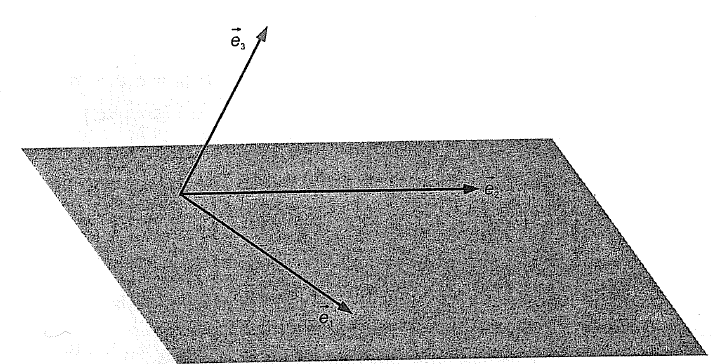
\includegraphics[scale=0.90]{b_v3.png}
	\caption{Base de um vetor em $\mathbb{R}^3$ \cite{camargo2005}, pg. 52.}
\end{figure}

Para analisar as propriedades da base de um espaço vetorial de forma generalizada, consideremos desta forma.

\noindent\textbf{Teorema 3:} Sejam $\mathbf{v}_1, \mathbf{v}_2, \ldots, \mathbf{v}_n \mid \mathbf{v} \neq 0$, estes que geram um espaço vetorial $\mathbf{V}$. Então, dentre este vetores podemos extrair uma base de $\mathbf{V}$.

Se $\mathbf{v}_1, \mathbf{v}_2, \ldots, \mathbf{v}_n$ são \textbf{LI}, então eles cumprem as condições para uma base, e não temos mais nada a fazer. Se $\mathbf{v}_1, \mathbf{v}_2, \ldots, \mathbf{v}_n$ são \textbf{LD}, então existe uma combinação linear deles, com algum coeficiente não zero, obtendo o vetor nulo

\begin{equation}
\mathbf{x}_1\mathbf{v}_1 + \mathbf{x}_2\mathbf{v}_2 + \ldots + \mathbf{x}_n\mathbf{v}_n = 0
\end{equation}

Se $\mathbf{x}_n \neq 0$. Então é possível escrever

\begin{equation}
\mathbf{v}_n = \frac{-\mathbf{x}_1}{\mathbf{x}_n}\mathbf{v}_1 + \frac{-\mathbf{x}_2}{\mathbf{x}_n}\mathbf{v}_2 + \ldots + \frac{-\mathbf{x}_{n -1}}{\mathbf{x}_n}\mathbf{v}_{n -1}
\end{equation}

ora, $\mathbf{v}_n$ é uma combinação linear de $\mathbf{v}_1, \ldots, \mathbf{v}_{n -1}$ e, portanto, $\mathbf{v}_1, \ldots, \mathbf{v}_{n -1}$ geram $\mathbf{V}$. Se $\mathbf{v}_1, \ldots, \mathbf{v}_{n -1}$ for \textbf{LD}, então existe uma combinação linear deles que dará o vetor nulo e com algum coeficiente $\neq 0$, portanto, é possível extrair o vetor que corresponde a este coeficiente. Se continuarmos, com as iterações, após uma quantidade $n$ de passos, obteremos um subconjunto de $\{\mathbf{v}_1, \ldots, \mathbf{v}_n\}$ formado por $r(r \leqslant n)$ vetores \textbf{LI} $\mathbf{v}_{i1}, \mathbf{v}_{i2}, \ldots, \mathbf{v}_{ir}$, que ainda geram $\mathbf{V}$, por fim, formará uma base.

\section{Dimensão}
A dimensão de um espaço vetorial $\mathbf{V}$ é o número de elementos de uma base para $V$, que denotamos por $\dim(\mathbf{V})$. Caso $\mathbf{V} = \{e\}$, o conjunto vazio é uma base para $V$ e $\dim(\mathbf{V}) = 0$. Qualquer base de um espaço vetorial tem sempre o mesmo número de elementos.

\noindent\textbf{Teorema 4:} Seja  $\mathbf{V}$ um espaço vetorial e $\{\mathbf{u}_1, \ldots, \mathbf{u}_n\}$ um conjunto de elementos que geram  $\mathbf{V}$. Então, dentre esses elementos podemos extrair uma base para $\mathbf{V}$.

\noindent\textbf{Teorema 5:} Seja $\mathbf{V}$ um espaço vetorial gerado por um conjunto finito de n elementos $\mathbf{u}_1, \mathbf{u}_2, \ldots, \mathbf{u}_n$. Então, qualquer conjunto linearmente independente em $\mathbf{V}$ possui no máximo $n$ elementos.

\noindent\textbf{Teorema 6:} Qualquer base de um espaço vetorial tem sempre o mesmo número (finito) de elementos.

\noindent\textbf{Teorema 7 (Completamento):} Qualquer conjunto de elementos \textbf{LI} de um espaço vetorial $\mathbf{V}$ de dimensão finita pode ser completado até formar uma base para $\mathbf{V}$.

\noindent\textbf{Teorema 8:} Seja $\mathbf{V}$ um espaço vetorial e $\mathbf{U}$ e $\mathbf{W}$ subespaços vetoriais de $\mathbf{V}$, então:

\centerline{$\dim(\mathbf{U} + \mathbf{W}) = \dim(\mathbf{U} + \dim(\mathbf{W}) - \dim(\mathbf{U} \cap \mathbf{W})$}
  
\noindent\textbf{Teorema 9:} Seja $\mathbf{V}$ um espaço vetorial e $\beta = \{\mathbf{u}_1, \ldots,\mathbf{u}_n\}$ uma base ordenada para $\mathbf{V}$, isto é, os elementos estão ordenados na ordem em que aparecem. Então, todo elemento de $\mathbf{V}$ pode ser escrito de maneira única como combinação linear de $\mathbf{u}_1, \ldots, \mathbf{u}_n$.

% _{m \times n}
% subinscrito
% _
% expoente com mais de um dígito
% x^{21}
